% GENERATED, edit the French unit or the translation table
\mxfront{stmg-bank-b}

% -----------------------------------------------------------------------------
% Chapitre 3 -- Fonction logarithme décimal
% -----------------------------------------------------------------------------
\mxexdef{15}{Isolate $10^x$, then take the logarithm}{%
Solve the following equations in $\R$. When a solution exists, give its exact value and then its value rounded to the nearest thousandth.
\begin{enumerate}[label=\alph*.]
\item $4\times10^x=\num{9,2}$
\item $7\times10^x-\num{1,5}=3\times10^x+\num{0,9}$
\item $\num{2,5}\times10^x+12=6-\num{0,5}\times10^x$
\item $10^{x+1}=50$ \quad (you may write $10^{x+1}=10\times10^x$)
\end{enumerate}
}{%
Method: gather the terms in $10^x$ on one side, isolate $10^x$, check that the right-hand side is strictly positive, then use: for $b>0$, $10^x=b \iff x=\log(b)$.
\begin{enumerate}[label=\alph*.]
\item $10^x=\dfrac{\num{9,2}}{4}=\num{2,3}>0$, so $x=\log(\num{2,3})\approx\num{0,362}$.
\item $7\times10^x-3\times10^x=\num{0,9}+\num{1,5}$, i.e. $4\times10^x=\num{2,4}$, so $10^x=\num{0,6}>0$ and $x=\log(\num{0,6})\approx-\num{0,222}$.
\item $\num{2,5}\times10^x+\num{0,5}\times10^x=6-12$, i.e. $3\times10^x=-6$, so $10^x=-2$. But $10^x>0$ for every real $x$: the equation has no solution.
\item $10\times10^x=50$, so $10^x=5>0$ and $x=\log(5)\approx\num{0,699}$. (Another way: $x+1=\log(50)$, so $x=\log(50)-1=\log(5)$.)
\end{enumerate}
Recommended calculator check: $10^{\num{0,362}}\approx\num{2,30}$ and $10^{-\num{0,222}}\approx\num{0,60}$.
}{4}

\mxexdef{16}{Sign of a logarithm and comparison}{%
Recall that the function $\log$ is strictly increasing on $\intoo{0}{+\infty}$ and that $\log(1)=0$.
\begin{enumerate}
\item Without a calculator, give the sign of each of the following numbers, with a justification:
\begin{enumerate}[label=\alph*.]
\item $\log(\num{0,9})$ ;
\item $\log\!\left(\dfrac{4}{3}\right)$ ;
\item $\log(CM)$, where $CM$ is the multiplier associated with an increase of $\pc{0,2}$.
\end{enumerate}
\item Without a calculator, compare $\log(\num{0,35})$ and $\log(\num{0,53})$.
\end{enumerate}
}{%
\begin{enumerate}
\item For $a>0$: if $a>1$ then $\log(a)>\log(1)=0$; if $0<a<1$ then $\log(a)<0$ (since $\log$ is strictly increasing).
\begin{enumerate}[label=\alph*.]
\item $0<\num{0,9}<1$, so $\log(\num{0,9})<0$ (about $-\num{0,046}$).
\item $\dfrac43>1$, so $\log\!\left(\dfrac43\right)>0$ (about $\num{0,125}$).
\item $CM=1+\dfrac{\num{0,2}}{100}=\num{1,002}>1$, so $\log(\num{1,002})>0$ (about $\num{0,000}\,87$: very close to $0$ but positive).
\end{enumerate}
\item $0<\num{0,35}<\num{0,53}$ and $\log$ is strictly increasing on $\intoo{0}{+\infty}$, so $\log(\num{0,35})<\log(\num{0,53})$. Both numbers are negative (arguments less than $1$); the one closer to $0$ is $\log(\num{0,53})$.
\end{enumerate}
}{3}

\mxexdef{17}{Condense an expression into one logarithm}{%
Write each of the following numbers in the form $\log(A)$, where $A$ is a strictly positive real number to be given as an integer or a fraction. When possible, give the exact value of the number.
\begin{enumerate}[label=\alph*.]
\item $\log(6)+\log(5)-\log(3)$
\item $2\log(4)-\log(8)$
\item $\log(5)+\log(11)$
\item $2\log(3)-3\log(2)$
\item $\log(40)-\log(8)+2\log(2)$
\end{enumerate}
}{%
We use, for $a,b>0$ and any natural number $n$: $\log(a)+\log(b)=\log(ab)$, $\log(a)-\log(b)=\log\!\left(\dfrac ab\right)$ and $n\log(a)=\log(a^n)$. All the arguments are strictly positive.
\begin{enumerate}[label=\alph*.]
\item $\log(6)+\log(5)-\log(3)=\log\!\left(\dfrac{6\times5}{3}\right)=\log(10)=1$.
\item $2\log(4)-\log(8)=\log(4^2)-\log(8)=\log\!\left(\dfrac{16}{8}\right)=\log(2)$.
\item $\log(5)+\log(11)=\log(55)$.
\item $2\log(3)-3\log(2)=\log(3^2)-\log(2^3)=\log\!\left(\dfrac98\right)$.
\item $\log(40)-\log(8)+2\log(2)=\log\!\left(\dfrac{40\times2^2}{8}\right)=\log(20)$.
\end{enumerate}
Error to point out: $\log(5)+\log(11)$ is not $\log(16)$; a sum of logarithms corresponds to a product of the arguments.
}{4}

\mxexdef{18}{Threshold algorithm for a change over time}{%
A delivery company buys a van for $\num{38000}$~€. Its value is estimated to fall by $\pc{15}$ each year. The company will sell the van as soon as its value becomes strictly less than $\num{10000}$~€.
Let $V$ be the value of the van (in euros) and $N$ the number of years since the purchase.
\begin{center}
\begin{tabular}{|l|}
\hline
$V\leftarrow\num{38000}$\\
$N\leftarrow0$\\
While $V\ \ldots\ldots\ldots$\\
\mxtab $V\leftarrow\ldots\ldots\ldots$\\
\mxtab $N\leftarrow N+1$\\
End While\\
\hline
\end{tabular}
\end{center}
\begin{enumerate}
\item Complete the algorithm so that, at the end of its execution, the variable $N$ contains the number of years after which the van will be sold.
\item Using the calculator (table of values), run the algorithm and find the value of $N$ obtained. Give the value of the van when it is sold, rounded to the nearest euro.
\item Write this program in Python, run it and compare with the result of question 2.
\end{enumerate}
}{%
\begin{enumerate}
\item A $\pc{15}$ decrease corresponds to the multiplier $1-\num{0,15}=\num{0,85}$. We repeat as long as the value has not yet fallen below the threshold: “While $V\geqslant\num{10000}$” and “$V\leftarrow\num{0,85}\times V$”.
\item Successive values rounded to the nearest euro: $N=6$: $\num{14332}$~€; $N=7$: $\num{12182}$~€; $N=8$: $\num{10355}$~€; $N=9$: $\num{8801}$~€.
Since $\num{38000}\times\num{0,85}^8\approx\num{10355}\geqslant\num{10000}$ and $\num{38000}\times\num{0,85}^9\approx\num{8801}<\num{10000}$, the loop stops with $N=9$: the van will be sold after $9$ years, for a value of about $\num{8801}$~€.
\item A possible program:\\
\texttt{V = 38000}\\
\texttt{N = 0}\\
\texttt{while V >= 10000:}\\
\mxtab \texttt{V = 0.85 * V}\\
\mxtab \texttt{N = N + 1}\\
\texttt{print(N, V)}\\
The program displays $9$ and about $\num{8801,44}$, which confirms question 2. Stress the decimal point in Python and the indentation of the loop block.
\end{enumerate}
}{5}

\mxexdef{19}{Doubling time and overtaking}{%
An online shop A received $\num{2500}$ orders in January 2026. This number is assumed to increase by $\pc{7}$ per month. Let $a_n$ be the number of orders $n$ months after January 2026.
\begin{enumerate}
\item
\begin{enumerate}[label=\alph*.]
\item Express $a_n$ in terms of $n$.
\item After how many months will the monthly number of orders have doubled?
\item After how many months will it have quadrupled? Is this result twice the previous one? Explain.
\end{enumerate}
\item A competing shop B received $\num{4000}$ orders in January 2026, with an increase of $\pc{3}$ per month. From how many months on will shop A have more monthly orders than shop B? In which month will this happen?
\end{enumerate}
}{%
\begin{enumerate}
\item
\begin{enumerate}[label=\alph*.]
\item An increase of $\pc{7}$ corresponds to the multiplier $\num{1,07}$: $a_n=\num{2500}\times\num{1,07}^n$.
\item $a_n\geqslant\num{5000}\iff\num{1,07}^n\geqslant2\iff n\log(\num{1,07})\geqslant\log(2)\iff n\geqslant\dfrac{\log(2)}{\log(\num{1,07})}$, because $\log(\num{1,07})>0$ (the inequality keeps its direction). Now $\dfrac{\log 2}{\log \num{1,07}}\approx\num{10,24}$: $11$ months are needed. Check: $\num{1,07}^{10}\approx\num{1,967}<2$ and $\num{1,07}^{11}\approx\num{2,105}\geqslant2$.
\item $\num{1,07}^n\geqslant4\iff n\geqslant\dfrac{\log(4)}{\log(\num{1,07})}\approx\num{20,49}$: $21$ months are needed ($\num{1,07}^{20}\approx\num{3,870}$ and $\num{1,07}^{21}\approx\num{4,141}$). Since $\log(4)=2\log(2)$, the exact threshold is indeed doubled ($\num{20,49}=2\times\num{10,24}$), but rounding up to the next integer happens only once: $21$, not $2\times11=22$.
\end{enumerate}
\item We look for $n$ such that $\num{2500}\times\num{1,07}^n>\num{4000}\times\num{1,03}^n$. Dividing by $\num{2500}\times\num{1,03}^n>0$: $\left(\dfrac{\num{1,07}}{\num{1,03}}\right)^n>\num{1,6}$. Since $\dfrac{\num{1,07}}{\num{1,03}}>1$, its logarithm is positive and $n>\dfrac{\log(\num{1,6})}{\log(\num{1,07}/\num{1,03})}\approx\num{12,34}$. Hence $n=13$: check $a_{12}\approx\num{5630}<\num{5703}$ and $a_{13}\approx\num{6025}>\num{5874}$. Shop A will overtake shop B in February 2027 ($13$ months after January 2026).
\end{enumerate}
}{5}

\mxexdef{20}{Finding a rate: equation $x^n=b$}{%
The retail price of a solar panel model went from $420$~€ in March 2021 to $260$~€ in September 2025, a period of $4$ years and $6$ months. The price is assumed to have changed at a constant annual rate $t$.
\begin{enumerate}
\item Justify that $(1+t)^{\num{4,5}}=\dfrac{260}{420}$.
\item Deduce $t$, rounded to $\pc{0,1}$. Interpret the sign of the result.
\item A second model costs $395$~€ today. If its price changes at the same annual rate, what will its price be in $2$ years and $3$ months? Round to the nearest euro.
\item The manufacturer of this second model would rather reach a price of $300$~€ in $2$ years and $3$ months. What constant annual rate should it apply? Round to $\pc{0,1}$.
\end{enumerate}
}{%
\begin{enumerate}
\item Over $\num{4,5}$ years, the price is multiplied by $(1+t)^{\num{4,5}}$, so $420(1+t)^{\num{4,5}}=260$, i.e. $(1+t)^{\num{4,5}}=\dfrac{260}{420}\approx\num{0,619}$.
\item $1+t>0$, so $1+t=\left(\dfrac{260}{420}\right)^{1/\num{4,5}}\approx\num{0,8989}$, hence $t\approx-\num{0,101}$, i.e. $t\approx-\pc{10,1}$. The rate is negative: the price fell on average by about $\pc{10,1}$ per year. Check: $420\times\num{0,8989}^{\num{4,5}}\approx260$.
\item $2$ years and $3$ months $=\num{2,25}$ years. Price: $395(1+t)^{\num{2,25}}$. Keeping the exact value of $1+t$ in memory: $395\times\left(\dfrac{260}{420}\right)^{\num{2,25}/\num{4,5}}=395\times\left(\dfrac{260}{420}\right)^{\num{0,5}}\approx395\times\num{0,7868}\approx\num{310,78}$. The price would be about $311$~€.
\item We solve $395(1+t')^{\num{2,25}}=300$, i.e. $(1+t')^{\num{2,25}}=\dfrac{300}{395}\approx\num{0,7595}$, so $1+t'=\left(\dfrac{300}{395}\right)^{1/\num{2,25}}\approx\num{0,8849}$ and $t'\approx-\pc{11,5}$. A decrease of about $\pc{11,5}$ per year would be needed.
\end{enumerate}
Remark: using a value of $t$ rounded too early slightly changes the results (for example $395\times\num{0,899}^{\num{2,25}}\approx\num{310,85}$); keep the value in memory.
}{4}

\mxexdef{21}{Using a formula $\log(N)/\log(2)$}{%
In a laboratory, a cell culture grows by successive divisions: at each generation, the number of cells doubles. When the number of cells goes from $N_0$ to $N$, the number of generations that have elapsed is
\[
g=\frac{\log\!\left(\dfrac{N}{N_0}\right)}{\log(2)}.
\]
For example, going from $1$ to $8$ cells corresponds to $g=\dfrac{\log(8)}{\log(2)}=3$ generations.
\begin{enumerate}
\item A culture goes from $\num{1000}$ to $\num{64000}$ cells. How many generations have elapsed?
\item Another culture goes from $500$ to $\num{128000}$ cells. Same question.
\item A culture of $\num{1000}$ cells develops for $\num{9,5}$ generations. About how many cells does it contain?
\item Starting from a single cell, how many cells are obtained after $20$ generations?
\item A laboratory starts from $\num{1000}$ cells and wants to obtain $\num{1000000000}$. How many generations are needed? Given that one generation lasts $30$ minutes, how much time should be planned?
\end{enumerate}
}{%
\begin{enumerate}
\item $\dfrac{N}{N_0}=64=2^6$, so $g=\dfrac{\log(2^6)}{\log(2)}=\dfrac{6\log(2)}{\log(2)}=6$ generations.
\item $\dfrac{N}{N_0}=\dfrac{\num{128000}}{500}=256=2^8$, so $g=8$ generations.
\item $g=\num{9,5}$ gives $\log\!\left(\dfrac{N}{\num{1000}}\right)=\num{9,5}\log(2)$, so $\dfrac{N}{\num{1000}}=10^{\num{9,5}\log(2)}=2^{\num{9,5}}\approx\num{724,08}$. Thus $N\approx\num{724000}$ cells.
\item $N=2^{20}=\num{1048576}$ cells, i.e. about one million.
\item $\dfrac{N}{N_0}=10^6$, so $g=\dfrac{\log(10^6)}{\log(2)}=\dfrac{6}{\log(2)}\approx\num{19,93}$: $20$ complete generations are needed. Time: $20\times30=600$ minutes, i.e. about $10$ hours.
\end{enumerate}
}{5}

\mxexdef{22}{Number of digits of an integer}{%
We look for a method to find the number of digits of a natural number $N\geqslant1$ without writing it out in full. The integer part of a real number $y\geqslant0$ is the greatest integer less than or equal to $y$; it is denoted $E(y)$.
\begin{enumerate}
\item Let $N=\num{4718}$.
\begin{enumerate}[label=\alph*.]
\item Bound $N$ between two consecutive powers of $10$. Deduce bounds for $\log(N)$ between two consecutive integers.
\item Compare $E(\log N)$ with the number of digits of $N$.
\end{enumerate}
\item An integer $N$ is written with $15$ digits.
\begin{enumerate}[label=\alph*.]
\item Bound $N$ between two consecutive powers of $10$, then $\log(N)$ between two consecutive integers.
\item What is $E(\log N)$?
\end{enumerate}
\item State a rule giving the number of digits of $N$ from $\log(N)$. Test it on $N=\num{1000}$.
\item Use this rule to find the number of digits of: a. $3^{100}$; b. $2^{64}$; c. $365\times10^{15}$.
\item A password is made of $12$ characters, each chosen from $62$ symbols ($26$ lower-case letters, $26$ upper-case letters, $10$ digits). There are $62^{12}$ possible passwords. How many digits does this number have?
\end{enumerate}
}{%
\begin{enumerate}
\item
\begin{enumerate}[label=\alph*.]
\item $10^3\leqslant\num{4718}<10^4$. Since $\log$ is strictly increasing, $3\leqslant\log(\num{4718})<4$ (we find $\log(\num{4718})\approx\num{3,674}$).
\item $E(\log N)=3$ and $N$ has $4$ digits: number of digits $=E(\log N)+1$.
\end{enumerate}
\item
\begin{enumerate}[label=\alph*.]
\item The smallest $15$-digit integer is $10^{14}$ and the smallest $16$-digit integer is $10^{15}$: $10^{14}\leqslant N<10^{15}$, so $14\leqslant\log(N)<15$.
\item $E(\log N)=14$, and $14+1=15$ digits.
\end{enumerate}
\item If $N$ has $k$ digits, $10^{k-1}\leqslant N<10^k$, so $k-1\leqslant\log(N)<k$: $E(\log N)=k-1$. Rule: \emph{the number of digits of $N$ is $E(\log N)+1$}. For $N=\num{1000}$: $\log(\num{1000})=3$, $E(3)+1=4$ digits, which is correct.
\item a. $\log(3^{100})=100\log(3)\approx\num{47,71}$: $47+1=48$ digits.\\
b. $\log(2^{64})=64\log(2)\approx\num{19,27}$: $20$ digits (indeed $2^{64}=\num{18446744073709551616}$).\\
c. $\log(365\times10^{15})=\log(365)+15\approx\num{17,56}$: $18$ digits.
\item $\log(62^{12})=12\log(62)\approx\num{21,51}$: $62^{12}$ is written with $22$ digits (about $\num{3,2}\times10^{21}$ passwords).
\end{enumerate}
}{6}

% -----------------------------------------------------------------------------
% Chapitre 4 -- Fonction inverse
% -----------------------------------------------------------------------------
\mxexdef{23}{Table of values and plotting hyperbolas}{%
Consider the functions $f$ and $g$ defined on $\R^{*}=\R\setminus\{0\}$ by
$f(x)=-\dfrac{2}{x}$ and $g(x)=1+\dfrac{3}{x}$.
\begin{enumerate}
\item Explain why $0$ does not belong to the domain of these functions.
\item Complete the table of values (values rounded to the nearest hundredth if necessary).
\begin{center}\small
\begin{tabular}{|c|*{10}{c|}}
\hline
$x$ & $-4$ & $-3$ & $-2$ & $-1$ & $-\num{0,5}$ & $\num{0,5}$ & $1$ & $2$ & $3$ & $4$\\
\hline
$f(x)$ & & & & & & & & & & \\
\hline
$g(x)$ & & & & & & & & & & \\
\hline
\end{tabular}
\end{center}
\item Plot the points and draw the curves $\mathcal{C}_f$ and $\mathcal{C}_g$ on the grid below.
\begin{center}
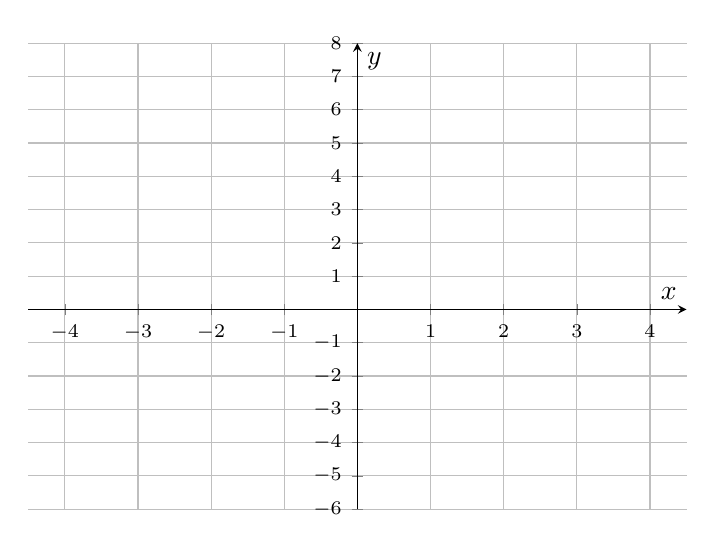
\begin{tikzpicture}
\begin{axis}[width=.82\linewidth,height=7.5cm,axis lines=middle,xmin=-4.5,xmax=4.5,ymin=-6,ymax=8,
  xtick={-4,...,4},ytick={-6,...,8},grid=major,xlabel={$x$},ylabel={$y$},tick label style={font=\scriptsize}]
\end{axis}
\end{tikzpicture}
\end{center}
\item Show that, for every non-zero real $x$, $f(-x)=-f(x)$. Which symmetry of $\mathcal{C}_f$ does this express? For each curve, give the lines it gets closer and closer to (asymptotes).
\end{enumerate}
}{%
\begin{enumerate}
\item Computing $\dfrac2x$ or $\dfrac3x$ requires dividing by $x$; division by $0$ is impossible. The domain is $\R^{*}=\intoo{-\infty}{0}\cup\intoo{0}{+\infty}$.
\item
\begin{center}\small
\begin{tabular}{|c|*{10}{c|}}
\hline
$x$ & $-4$ & $-3$ & $-2$ & $-1$ & $-\num{0,5}$ & $\num{0,5}$ & $1$ & $2$ & $3$ & $4$\\
\hline
$f(x)$ & $\num{0,5}$ & $\num{0,67}$ & $1$ & $2$ & $4$ & $-4$ & $-2$ & $-1$ & $-\num{0,67}$ & $-\num{0,5}$\\
\hline
$g(x)$ & $\num{0,25}$ & $0$ & $-\num{0,5}$ & $-2$ & $-5$ & $7$ & $4$ & $\num{2,5}$ & $2$ & $\num{1,75}$\\
\hline
\end{tabular}
\end{center}
\item
\begin{center}
\begin{tikzpicture}
\begin{axis}[width=.82\linewidth,height=7.5cm,axis lines=middle,xmin=-4.5,xmax=4.5,ymin=-6,ymax=8,
  xtick={-4,...,4},ytick={-6,...,8},grid=major,xlabel={$x$},ylabel={$y$},tick label style={font=\scriptsize}]
\addplot[mxteacher,very thick,samples=100,domain=-4.5:-0.34]{-2/x};
\addplot[mxteacher,very thick,samples=100,domain=0.25:4.5]{-2/x};
\addplot[mxwarn,very thick,samples=100,domain=-4.5:-0.43]{1+3/x};
\addplot[mxwarn,very thick,samples=100,domain=0.43:4.5]{1+3/x};
\addplot[mxwarn,dashed] coordinates {(-4.5,1)(4.5,1)};
\node[mxteacher,anchor=west] at (axis cs:2.2,-1.8) {$\mathcal{C}_f$};
\node[mxwarn,anchor=west] at (axis cs:2.2,3.2) {$\mathcal{C}_g$};
\end{axis}
\end{tikzpicture}
\end{center}
\item $f(-x)=-\dfrac{2}{-x}=\dfrac2x=-f(x)$. The points with coordinates $\pt{x;f(x)}$ and $\pt{-x;-f(x)}$ are symmetric about the origin: $\mathcal{C}_f$ is symmetric about the origin $O$. Asymptotes: for $\mathcal{C}_f$, the lines with equations $x=0$ and $y=0$; for $\mathcal{C}_g$, the lines with equations $x=0$ and $y=1$ (the curve of $g$ is symmetric about the point $\pt{0;1}$, since $g(-x)+g(x)=2$).
\end{enumerate}
}{5}

\mxexdef{24}{End behaviour and asymptotes}{%
Let $h$ be the function defined on $\R^{*}$ by $h(x)=-1+\dfrac{5}{x}$.
\begin{enumerate}
\item Compute $h(x)$ for $x\in\ens{-\num{10000};-\num{1000};-100;100;\num{1000};\num{10000}}$. What can be conjectured about $h(x)$ when $x$ becomes very large in absolute value? Which asymptote can be deduced?
\item Compute $h(x)$ for $x\in\ens{-\num{0,1};-\num{0,01};-\num{0,001};\num{0,001};\num{0,01};\num{0,1}}$. Describe the behaviour of $h(x)$ when $x$ gets close to $0$, first through negative values, then through positive values. Which asymptote can be deduced?
\item Compute $h(-5)$, $h(-1)$, $h(1)$ and $h(5)$, then sketch the curve of $h$ and its asymptotes on the grid below.
\begin{center}
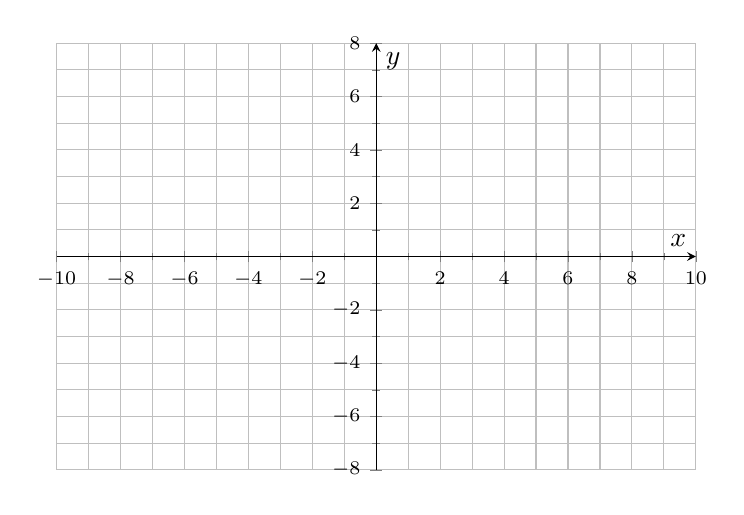
\begin{tikzpicture}
\begin{axis}[width=.8\linewidth,height=7cm,axis lines=middle,xmin=-10,xmax=10,ymin=-8,ymax=8,
  xtick={-10,-8,...,10},ytick={-8,-6,...,8},minor tick num=1,grid=both,xlabel={$x$},ylabel={$y$},tick label style={font=\scriptsize}]
\end{axis}
\end{tikzpicture}
\end{center}
\item Application. A training organisation rents a room for $450$~€ per day and spends $12$~€ on meals per participant. For $x$ participants ($x\geqslant1$), the average cost per participant is $c(x)=12+\dfrac{450}{x}$ (in euros).
\begin{enumerate}[label=\alph*.]
\item Compute $c(10)$, $c(50)$ and $c(150)$.
\item Which value does the average cost get closer to when the number of participants becomes very large? Can it fall below $12$~€? Justify.
\end{enumerate}
\end{enumerate}
}{%
\begin{enumerate}
\item $h(-\num{10000})=-\num{1,000}\,5$; $h(-\num{1000})=-\num{1,005}$; $h(-100)=-\num{1,05}$; $h(100)=-\num{0,95}$; $h(\num{1000})=-\num{0,995}$; $h(\num{10000})=-\num{0,999}\,5$. When $|x|$ becomes very large, $\dfrac5x$ gets close to $0$, so $h(x)$ gets close to $-1$ (from below at $-\infty$, from above at $+\infty$). The line with equation $y=-1$ is a horizontal asymptote.
\item $h(-\num{0,1})=-51$; $h(-\num{0,01})=-501$; $h(-\num{0,001})=-\num{5001}$; $h(\num{0,001})=\num{4999}$; $h(\num{0,01})=499$; $h(\num{0,1})=49$. When $x$ gets close to $0$ through negative values, $h(x)$ is negative and as large as we like in absolute value ($h(x)\to-\infty$); through positive values, $h(x)\to+\infty$. The line with equation $x=0$ is a vertical asymptote.
\item $h(-5)=-2$, $h(-1)=-6$, $h(1)=4$, $h(5)=0$.
\begin{center}
\begin{tikzpicture}
\begin{axis}[width=.8\linewidth,height=7cm,axis lines=middle,xmin=-10,xmax=10,ymin=-8,ymax=8,
  xtick={-10,-8,...,10},ytick={-8,-6,...,8},minor tick num=1,grid=both,xlabel={$x$},ylabel={$y$},tick label style={font=\scriptsize}]
\addplot[mxteacher,very thick,samples=120,domain=-10:-0.72]{-1+5/x};
\addplot[mxteacher,very thick,samples=120,domain=0.56:10]{-1+5/x};
\addplot[mxwarn,dashed,thick] coordinates {(-10,-1)(10,-1)};
\addplot[only marks,mark=*,mxteacher] coordinates {(-5,-2)(-1,-6)(1,4)(5,0)};
\end{axis}
\end{tikzpicture}
\end{center}
\item
\begin{enumerate}[label=\alph*.]
\item $c(10)=12+45=57$~€ ; $c(50)=12+9=21$~€ ; $c(150)=12+3=15$~€.
\item When $x$ becomes very large, $\dfrac{450}{x}$ gets close to $0$: the average cost gets close to $12$~€ (asymptote $y=12$). Since $\dfrac{450}{x}>0$ for $x>0$, we always have $c(x)>12$: the average cost never falls below $12$~€, as the fixed cost of the room is shared among the participants without disappearing.
\end{enumerate}
\end{enumerate}
}{5}

\mxexdef{25}{Differentiate a polynomial plus $k/x$}{%
Compute the derivative of each of the following functions, defined on $\R^{*}$.
\begin{enumerate}[label=\alph*.]
\item $f(x)=5x+2-\dfrac{3}{x}$
\item $g(x)=-4x+7+\dfrac{6}{x}$
\item $h(x)=2x^3-5x^2+\dfrac{1}{x}$
\item $k(x)=\dfrac12x^2+4x-\dfrac{8}{x}$
\item $p(x)=\dfrac{x^2+2}{x}$ \quad (first write $p(x)$ in the form $x+\dfrac{a}{x}$, then give $p'(x)$ as a single quotient)
\end{enumerate}
}{%
We use: $(ax^n)'=nax^{n-1}$, the derivative of a constant is zero and, for $x\neq0$, $\left(\dfrac{k}{x}\right)'=k\times\left(-\dfrac1{x^2}\right)=-\dfrac{k}{x^2}$.
\begin{enumerate}[label=\alph*.]
\item $f'(x)=5-\left(-\dfrac{3}{x^2}\right)=5+\dfrac{3}{x^2}$.
\item $g'(x)=-4-\dfrac{6}{x^2}$.
\item $h'(x)=6x^2-10x-\dfrac{1}{x^2}$.
\item $k'(x)=x+4+\dfrac{8}{x^2}$.
\item $p(x)=\dfrac{x^2}{x}+\dfrac{2}{x}=x+\dfrac2x$, so $p'(x)=1-\dfrac2{x^2}=\dfrac{x^2-2}{x^2}$.
\end{enumerate}
Common error: writing $\left(\dfrac{3}{x}\right)'=\dfrac{3}{x^2}$, forgetting the “$-$” sign.
}{5}

\mxexdef{26}{Factorised derivative, sign and variations}{%
Let $f$ be the function defined on $\R^{*}$ by $f(x)=9x-2+\dfrac{4}{x}$.
\begin{enumerate}
\item Show that, for every non-zero real $x$, $f'(x)=\dfrac{(3x-2)(3x+2)}{x^2}$.
\item Study the sign of $f'(x)$ on $\R^{*}$ using a sign table.
\item Deduce the table of variations of $f$, including the values of $f\!\left(-\dfrac23\right)$ and $f\!\left(\dfrac23\right)$.
\item Compare $f\!\left(-\dfrac23\right)$ and $f\!\left(\dfrac23\right)$. Can a local maximum be less than a local minimum? Explain using the table.
\end{enumerate}
}{%
\begin{enumerate}
\item $f'(x)=9-\dfrac{4}{x^2}=\dfrac{9x^2-4}{x^2}=\dfrac{(3x-2)(3x+2)}{x^2}$ (identity $a^2-b^2=(a-b)(a+b)$ with $a=3x$, $b=2$).
\item $x^2>0$ for $x\neq0$: the sign of $f'(x)$ is that of $(3x-2)(3x+2)$. $3x+2=0\iff x=-\dfrac23$; $3x-2=0\iff x=\dfrac23$.
\[
\begin{array}{|c|ccccccccc|}
\hline
x & -\infty & & -\frac23 & & 0 & & \frac23 & & +\infty\\ \hline
3x+2 & & - & 0 & + & \| & + & & + & \\
3x-2 & & - & & - & \| & - & 0 & + & \\
x^2 & & + & & + & 0 & + & & + & \\ \hline
f'(x) & & + & 0 & - & \| & - & 0 & + & \\ \hline
\end{array}
\]
\item $f\!\left(-\dfrac23\right)=-6-2-6=-14$ and $f\!\left(\dfrac23\right)=6-2+6=10$.
\[
\begin{array}{|c|ccccccccc|}
\hline
x & -\infty & & -\frac23 & & 0 & & \frac23 & & +\infty\\ \hline
f(x) & & \nearrow & -14 & \searrow & \| & \searrow & 10 & \nearrow & \\ \hline
\end{array}
\]
$f$ is increasing on $\left]-\infty;-\dfrac23\right]$, decreasing on $\left[-\dfrac23;0\right[$ and on $\left]0;\dfrac23\right]$, increasing on $\left[\dfrac23;+\infty\right[$.
\item $-14<10$: the local maximum (reached at $-\dfrac23$, on $\intoo{-\infty}{0}$) is less than the local minimum (reached at $\dfrac23$, on $\intoo{0}{+\infty}$). This is not a contradiction: they are local extrema on two intervals separated by the forbidden value $0$, where the curve “jumps” (vertical asymptote).
\end{enumerate}
}{4}

\mxexdef{27}{Always-positive derivative and sign of a quotient}{%
Let $h$ be the function defined on $\R^{*}$ by $h(x)=2x-3-\dfrac{5}{x}$.
\begin{enumerate}
\item Show that, for every non-zero real $x$, $h'(x)=\dfrac{2x^2+5}{x^2}$.
\item Study the sign of $h'(x)$ and deduce the variations of $h$.
\item Compute $h(-1)$ and $h(1)$. Can we say that “$h$ is increasing on $\R^{*}$”? Explain.
\item Show that, for every non-zero real $x$, $h(x)=\dfrac{(2x-5)(x+1)}{x}$. Draw the sign table of $h(x)$, then solve the inequality $h(x)\geqslant0$.
\end{enumerate}
}{%
\begin{enumerate}
\item $h'(x)=2-\left(-\dfrac{5}{x^2}\right)=2+\dfrac{5}{x^2}=\dfrac{2x^2+5}{x^2}$.
\item For $x\neq0$: $2x^2+5\geqslant5>0$ and $x^2>0$, so $h'(x)>0$. The function $h$ is strictly increasing on $\intoo{-\infty}{0}$ and strictly increasing on $\intoo{0}{+\infty}$.
\[
\begin{array}{|c|ccccc|}
\hline
x & -\infty & & 0 & & +\infty\\ \hline
h'(x) & & + & \| & + & \\ \hline
h(x) & & \nearrow & \| & \nearrow & \\ \hline
\end{array}
\]
\item $h(-1)=-2-3+5=0$ and $h(1)=2-3-5=-6$. We have $-1<1$ but $h(-1)>h(1)$: $h$ is not increasing on the whole of $\R^{*}$. It is increasing on each of the two intervals, separately.
\item $\dfrac{(2x-5)(x+1)}{x}=\dfrac{2x^2-3x-5}{x}=2x-3-\dfrac5x=h(x)$. Critical values: $-1$, $0$ (forbidden value) and $\dfrac52$.
\[
\begin{array}{|c|ccccccccc|}
\hline
x & -\infty & & -1 & & 0 & & \frac52 & & +\infty\\ \hline
2x-5 & & - & & - & & - & 0 & + & \\
x+1 & & - & 0 & + & & + & & + & \\
x & & - & & - & 0 & + & & + & \\ \hline
h(x) & & - & 0 & + & \| & - & 0 & + & \\ \hline
\end{array}
\]
The solution set of $h(x)\geqslant0$ is $\intfo{-1}{0}\cup\left[\dfrac52;+\infty\right[$ ($0$ is excluded as a forbidden value). Check: $h(-\num{0,5})=6>0$, $h(1)=-6<0$, $h(3)=\dfrac43>0$.
\end{enumerate}
}{5}

\mxexdef{28}{Derivative and variations of the reciprocal function}{%
Let $f$ be the reciprocal function, defined on $\R^{*}$ by $f(x)=\dfrac1x$.
\begin{enumerate}
\item Let $h$ be a non-zero real number, with $h\neq-2$. Show that the rate of change of $f$ between $2$ and $2+h$ is
$\dfrac{f(2+h)-f(2)}{h}=-\dfrac{1}{2(2+h)}$. Letting $h$ tend to $0$, deduce $f'(2)$.
\item We admit that, for every non-zero real $x$, $f'(x)=-\dfrac1{x^2}$. Check consistency with question 1, then compute $f'(-1)$ and $f'(\num{0,5})$.
\item Study the sign of $f'(x)$ and draw the table of variations of $f$.
\item A student notices that $-2<3$ and $f(-2)<f(3)$, and claims that this contradicts the fact that $f$ is decreasing. What should we answer?
\end{enumerate}
}{%
\begin{enumerate}
\item $f(2+h)-f(2)=\dfrac1{2+h}-\dfrac12=\dfrac{2-(2+h)}{2(2+h)}=\dfrac{-h}{2(2+h)}$. Dividing by $h\neq0$: $\dfrac{f(2+h)-f(2)}{h}=-\dfrac1{2(2+h)}$. When $h$ tends to $0$, this rate tends to $-\dfrac1{2\times2}=-\dfrac14$: $f'(2)=-\dfrac14$.
\item $-\dfrac1{2^2}=-\dfrac14$: consistent. $f'(-1)=-\dfrac1{(-1)^2}=-1$ and $f'(\num{0,5})=-\dfrac1{\num{0,25}}=-4$ (slopes of the tangents at these points).
\item For $x\neq0$, $x^2>0$, so $f'(x)=-\dfrac1{x^2}<0$.
\[
\begin{array}{|c|ccccc|}
\hline
x & -\infty & & 0 & & +\infty\\ \hline
f'(x) & & - & \| & - & \\ \hline
f(x) & & \searrow & \| & \searrow & \\ \hline
\end{array}
\]
$f$ is strictly decreasing on $\intoo{-\infty}{0}$ and strictly decreasing on $\intoo{0}{+\infty}$.
\item $f(-2)=-\num{0,5}$ and $f(3)\approx\num{0,33}$: indeed $f(-2)<f(3)$. There is no contradiction: $-2$ and $3$ are not in the same interval. The reciprocal function is decreasing on each interval separately, not on the whole of $\R^{*}$; images can be compared using the direction of variation only for two real numbers in the same interval.
\end{enumerate}
}{4}

\mxexdef{29}{Reading an average cost from a graph}{%
A company assembles between $10$ and $70$ electric bicycles per month. For $x$ bicycles assembled, let $C(x)$ be the average unit production cost, in euros. The curve of the function $C$ on $\intff{10}{70}$ is given below.
\begin{center}
\begin{tikzpicture}
\begin{axis}[width=.85\linewidth,height=7.5cm,xmin=10,xmax=70,ymin=650,ymax=1050,
  xtick={10,15,...,70},ytick={650,700,...,1050},minor y tick num=1,grid=both,
  xlabel={number of bicycles $x$},ylabel={$C(x)$ in €},tick label style={font=\scriptsize},label style={font=\small}]
\addplot[mxteacher,very thick,samples=150,domain=10:70]{8*x+200+7200/x};
\end{axis}
\end{tikzpicture}
\end{center}
\begin{enumerate}
\item Read the average unit cost when the company assembles $15$ bicycles, then $50$ bicycles.
\item For which production levels is the average unit cost equal to $800$~€?
\item What is the minimum average unit cost? For which production level is it reached?
\item We admit that $C(x)=8x+200+\dfrac{\num{7200}}{x}$. Compute $C'(x)$, check that $C'(x)=\dfrac{8(x-30)(x+30)}{x^2}$ and confirm the answer to question 3 by calculation.
\end{enumerate}
}{%
Require reading lines (dotted) and units; a graphical reading is approximate.
\begin{enumerate}
\item We read $C(15)\approx800$~€ and $C(50)\approx745$~€ (exact value with the formula of question 4: $744$~€).
\item Draw the line with equation $y=800$: it meets the curve at the points with abscissas $15$ and $60$. The average cost is $800$~€ for $15$ or $60$ bicycles.
\item The lowest point of the curve has coordinates about $\pt{30;680}$: minimum cost of about $680$~€ per bicycle, for $30$ bicycles per month.
\item $C'(x)=8-\dfrac{\num{7200}}{x^2}=\dfrac{8x^2-\num{7200}}{x^2}=\dfrac{8(x^2-900)}{x^2}=\dfrac{8(x-30)(x+30)}{x^2}$. On $\intff{10}{70}$, $x+30>0$ and $x^2>0$: $C'(x)$ has the sign of $x-30$, negative on $\intfo{10}{30}$ and positive on $\intof{30}{70}$. $C$ is decreasing on $\intff{10}{30}$ then increasing on $\intff{30}{70}$; its minimum is $C(30)=240+200+240=680$~€. Checks: $C(15)=120+200+480=800$ and $C(60)=480+200+120=800$.
\end{enumerate}
}{5}

\mxexdef{30}{Minimising an average cost with the derivative}{%
A composting site produces $x$ tonnes of compost each week, with $x\in\intff{2}{25}$. The total weekly production cost, in euros, is modelled by $C(x)=2x^2+40x+288$.
Let $f$ be the function giving the average production cost of one tonne: $f(x)=\dfrac{C(x)}{x}$.
\begin{enumerate}
\item Show that, for every $x\in\intff{2}{25}$, $f(x)=2x+40+\dfrac{288}{x}$.
\item Compute $f'(x)$ and show that, for every $x\in\intff{2}{25}$, $f'(x)=\dfrac{2(x-12)(x+12)}{x^2}$.
\item Study the sign of $f'(x)$ on $\intff{2}{25}$ and draw the table of variations of $f$ (including the values at the endpoints).
\item What is the minimum average cost of one tonne of compost? For which weekly production is it reached? What is the total cost of the week then?
\end{enumerate}
}{%
\begin{enumerate}
\item For $x\in\intff{2}{25}$, $x\neq0$: $f(x)=\dfrac{2x^2}{x}+\dfrac{40x}{x}+\dfrac{288}{x}=2x+40+\dfrac{288}{x}$.
\item $f'(x)=2-\dfrac{288}{x^2}=\dfrac{2x^2-288}{x^2}=\dfrac{2(x^2-144)}{x^2}=\dfrac{2(x-12)(x+12)}{x^2}$.
\item On $\intff{2}{25}$: $2>0$, $x+12>0$ and $x^2>0$, so $f'(x)$ has the sign of $x-12$: $f'(x)<0$ on $\intfo{2}{12}$, $f'(12)=0$, $f'(x)>0$ on $\intof{12}{25}$.
$f(2)=4+40+144=188$; $f(12)=24+40+24=88$; $f(25)=50+40+\num{11,52}=\num{101,52}$.
\[
\begin{array}{|c|ccccc|}
\hline
x & 2 & & 12 & & 25\\ \hline
f'(x) & & - & 0 & + & \\ \hline
f(x) & 188 & \searrow & 88 & \nearrow & \num{101,52}\\ \hline
\end{array}
\]
\item The minimum average cost is $88$~€ per tonne, reached for a production of $12$ tonnes per week. The total cost is then $C(12)=288+480+288=\num{1056}$~€ (check: $12\times88=\num{1056}$).
\end{enumerate}
}{4}
